Genbox is a tool for generating a number of tensor-product boxes, i.e., a set
of \(nelx \times nely \times nelz\) elements, where the locations of the vertices of the
elements are given as one-dimensional arrays of length \(nelx+1\), \(nely+1\), and
\(nelz+1\), respectively.  After running genbox, an output mesh file (.rea) is
created according to specifications in the input~.box file.

\subsection{Running genbox}

Before running genbox, ensure that the Nek5000 tools in {\tt Nek5000/tools}
are compiled and up-to-date.  Also ensure that the Nek5000 tools have been
added to your executable path (i.e., the {\tt \$PATH} variable).  See
section~\ref{ch:quick_start}) for information on compiling the Nek5000 tools.

To run genbox, type {\tt genbox} on the command line.  You will be prompted
for the filename of the input~.box file with the following message:

\begin{verbatim}
Enter the full name of the .box file, including the .box extension
\end{verbatim}

See Section~\ref{sec:box_file} for a description of the~.box file format.  A
successful genbox run will create a box.rea file (and a box.re2 file if
requested).  From here, you may use genmap to create a box.map file (see
Section~\ref{sec:genmap} for instructions on using genmap).  At any point in
this process, the box.xxx files may be moved and renamed using the script mvn
in {\tt Nek5000/bin/mvn}.  

\subsection{The~.box file format}\label{sec:box_file}

Genmap uses~.box files to describe geometries.  The box file includes a header
that is formatted the same for all geometries; a description that is formatted
for specific geometries; and a footer that is formatted the same for all
geometries.  In the~.box file, all lines beginning with the hash symbol
({\tt \#}) are comments and will be ignored.  {\em Genbox can only read
in 132 characters per line, so any line that exceeds this limit MUST be split
into 2 lines.}

\subsubsection{Header for all geometries}

\begin{description}

  \item[Line 1:] The name of an existing~.rea file that has the appropriate run
    parameters.  While the parameters can be modified later, it is important
    that the dimension of the~.rea file matches the dimension desired for the
    new files.

  \item[Line 2:] Indicates the spatial dimension. If less than zero, genbox will
    create an ASCII~.rea containing the runtime parameters and a binary~.re2
    file containing the mesh and boundary data.

  \item[Line 3:] The number of fields for this simulation, \(nfld\)
    (corresponding to velocity, heat transfer, etc.). Note that \(nfld\) must
    never be set to zero!

    \begin{itemize}

      \item If \(nfld<0\): genbox will create files that solve for only heat +
        \(nfld-1\) passive scalars and not for fluid. 

      \item If \(nfld>0\): genbox will solve for fluid, heat, and then
        \(nfld-2\) passive scalars.   
    
      \item If you intend to run MHD, \(nfld\) should be a decimal number of the
        format {\tt X.1} where the integer part {\tt X} is the number of
        fields and the decimal part {\tt .1} instructs genbox to look for
        the magnetic field properties.

    \end{itemize}

  \item[Line 4:] Indicates that a new box is starting and that the following
    lines will describe that box.  
    \begin{itemize}

      \item For normal, box geometries, this can be any string that doesn't
        start with a "c", "C", "m", "M", "y", or "Y".

      \item For annulus geometries with circular-only edges (and the option
        less than 360 degree), this line must start with a "c" or a "C".

      \item For annulus geometries with varying boundary shapes, this line must
        start with a "y" or a "Y".

      \item For geometries with varying segments of x,y,(z) distributions, this
        line must start with a "m" or "M".

    \end{itemize}

\end{description}

\subsubsection{Description for box geometries}

\begin{description}

  \item[Line 5:] The number of elements in the \(x\), \(y\) (and for 3D, \(z\))
    directions.  
    
    \begin{itemize}

      \item If these values are negative, genbox will automatically generate
        the element distribution along each axis. 

      \item If these values are positive, the user must explicitly provide the
        element distributions.  

    \end{itemize}
    

  \item[Lines 6, 7, (8 in 3D):] The distribution of elements in each
    spatial direction. Since there is a limit of 132 characters per line, it
    may be necessary to wrap these points across various lines.

    \begin{itemize}

      \item If the number of elements was less than zero, the user only
        supplies the start point \(x_0\), the ending point \(x_{nelx}\) and the
        ratio, or relative size, of each element progressing from left to
        right.  

      \item If the number of elements was greater than zero, each $nelx$ point
        in that direction, i.e., \(x_0, x_1, \ldots, x_{nelx}\) must be
        specified.

    \end{itemize}

\end{description}

\subsubsection{Description for circular-only annulus geometries}

\begin{description} 
  
  \item[Line 5:] The \(x\), \(y\), (and for 3D, \(z\)) center of the geometry.
    Note that this is an annulus geometry, so the \(x\) starting point cannot
    equal the center.

  \item[Line 6:] The number of elements in each direction \(nelx\), \(nely\),
    \(nelz\).

    \begin{itemize}

      \item If any are negative, genbox will automatically distribute the
        elements for the respective dimensions(s).

      \item If any are positive, genbox will look for user-specified elements
        for the respective dimension(s).

    \end{itemize}

  \item [Lines 7, 8, (9 in 3D):] The element distribution of each dimension.  The
    \(y\) dimension is given in degrees. For example, '0 360 1' would be a full
    circle with uniform distribution, and '90 180 1' would be a quarter-circle
    starting at the 90 degree point.

\end{description}

\subsubsection{Description for annulus geometries}

Note: For these geometries, genbox is currently setup for ASCII output only.

\begin{description}

  \item[Line 5:] Specifies the number of elements in each direction, \(nelx\),
    \(nely\), (and for 3D, \(nelz\)).

    \begin{itemize}

      \item If any are negative, genbox will automatically distribute the
        elements for this dimension.

      \item If any are positive, genbox will look for user-specified elements
        for this dimension.

    \end{itemize}

  \item[Line 6:] Coodinates of the center of the annulus, \((x0, y0)\). Since this
    is annulus geometry, \((x0,y0,z0)\) must not be the center.

  \item[Line 7:] String that specifies the cylinder type for each x-level of the
    annulus.  There must be \(nelx+1\) characters in this string.  The available
    characters are:

    \begin{description}
      \item[``c'':] curve boundary geometry
      \item[``o'':] octagon
      \item[``b'':] box (Cartesian)
    \end{description}

    When mixing curve (c) sides and box (b) sides, the elements on each level
    must not overflow into the next.  This will produce an error in genbox.  To
    fix this, the \(nelx\) points (or ratio) must be adjusted.  Furthermore,
    box-like sides work best with an even number of \(nely\) elements.

  \item[Lines 8, 9, (10 in 3D):] The coordinates of the elements.

    \begin{itemize}

      \item If the user gave a negative dimension, they only need to provide
        \(r0\), \(r1\), \(ratio\) (start, end, ratio) for this dimension.

      \item If the user gave a positive dimension, they will need to provide
        each point in this direction, i.e, \(r0, r0+1, \ldots, r1\) totaling the
        number of elements + 1.

    \end{itemize}

\end{description}

\subsubsection{Description for Multiple Segmented Geometries}

This feature allows users to enter a complex sequence of segments for each of
the \((x,y,z)\) directions. Each segment set is defined in \((x,y,z)\) sections.
Lines 5-8 describe the \(x\)-dimension, lines 9-12 the \(y\)-dimension,
and lines 13-16 the \(z\)-direction.

\begin{description}

  \item[Line 5:] The number of segments, \(nsegs\), in the \(x\)-direction.

  \item[Line 6:] The number of elements in each segment. There should be \(nsegs\)
    numbers, \\
    \((nelx_1, nelx_2, \ldots, nelx_{nsegs})\).

  \item[Line 7:] The start (and end) coordinates for each segment in this
    direction.  There should be \(nsegs+1\) numbers, \((x_0, x_1, \ldots,
    x_{nsegs})\).

  \item[Line 8:] The distribution of each segment. Uniform spacing corresponds
    to 1; otherwise a geometric sequence is generated.  In conclusion, a
    segment between \(x_{i-1}\) and \(x_i\) is filled with \(nelx_i\) elements
    determined by the geometric ratio given for that segment.

  \item[Lines 9-12:] Description of segments for \(y\)-dimension.  Follows the
    same format as lines 5-8.

  \item[Lines 13-16 (in 3D):] Description of segments for \(z\)-dimension.
    Follows the same format as lines 5-8.

\end{description}

\subsubsection{Footer for all geometries}

The last lines of the~.box file describe the boundary conditions.  There is one
line of boundary conditions for each fld field indicated (including MHD).  The
order of the boundary conditions are: west, east, south, north, bottom, top.
Genbox expects each boundary condition to be 3 characters followed by a comma,
so it is important maintain the proper spacing.  See Section~\ref{sec:boundary}
for available options {\em Note: there should be no blank lines at the end
  of the~.box file.  Extra whitespace will cause genbox to search for another
new tensor box data.}


% START WIP

% END WIP

\subsection{Example~.box files}

\subsubsection{Uniformly distributed mesh}

Suppose you wish to simulate flow through an axisymmetric pipe, of radius
\(R=0.5\) and length \(L=4\).  You estimate that you will need 3 elements in
radial (\(y\)) direction, and 5 in the \(x\) direction, as depicted in
Fig.~\ref{fig:mesh_axi1}.  This would be specified by the following input file
(called {\em pipe.box}) to genbox:

\begin{verbatim}
axisymmetric.rea
2                      spatial dimension
1                      number of fields
#
#    comments:   This is the box immediately behind the 
#                refined cylinder in Ugo's cyl+b.l. run.
#
#
#========================================================
#
Box 1                         Pipe
-5 -3                         Nelx  Nely
0.0   4.0   1.0               x0  x1   ratio
0.0   0.5   1.0               y0  y1   ratio
v  ,O  ,A  ,W  ,   ,          BC's:  (cbx0, cbx1, cby0, cby1, cbz0, cbz1)
\end{verbatim}
\begin{figure}
  \centering
  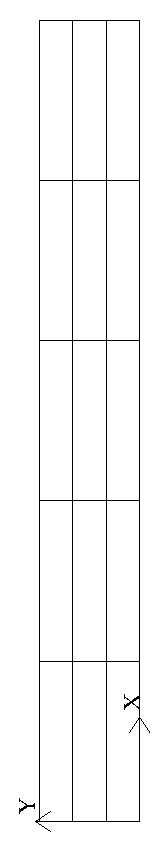
\includegraphics[width=0.8\textwidth]{Figs/mesh_axi1}
  \caption{Axisymmteric pipe mesh}
  \label{fig:mesh_axi1}
\end{figure}
\noindent
\begin{itemize}
  \item
    The first line of this file supplies the name of an existing 2D .rea file
    that has the appropriate run parameters (viscosity, timestep size, etc.).
    These parameters can be modified later, but it is important that 
    axisymmetric.rea be a 2D file, and not a 3D file.
  \item
    The second line indicates the number of fields for this simulation, in
    this case, just 1, corresponding to the velocity field (i.e., no heat 
    transfer).
  \item
    The next set of lines just shows how one can place comments into a genbox
    input file.
  \item
    The line that starts with ``Box'' indicates that a new box is starting,
    and that the following lines describe a typical box input.  Other possible
    key characters (the first character of Box, ``B'') are ``C'' and ``M'',
    more on those later.
  \item
    The first line after ``Box'' specifies the number of elements in the
    \(x\) and \(y\) directions.   The fact that these values are negative indicates
    that you want genbox to automatically generate the element distribution 
    along each axis, rather than providing it by hand.  (More on this below.)
  \item
    The next line specifies the distribution of the 5 elements in the \(x\) direction.
    The mesh starts at \(x=0\) and ends at \(x=4.0\).  The {\em ratio} indicates the
    relative size of each element, progressing from left to right.  Here, 
  \item
    The next line specifies the distribution of the 3 elements in the \(y\) direction,
    starting at \(y=0\) and going to \(y=0.5\).  Again, 
    {\em ratio}=1.0 indicates that the elements will be of uniform height.
  \item
    The last line specifies boundary conditions on each of the 4 sides of the
    box:  
    \begin{itemize}
      \item
        Lower-case {\em v} indicates that the left (\(x\)) boundary is to be a velocity
        boundary condition, with a user-specified distribution determined by 
        routine {\em userbc} in the .usr file.  (Upper-case \(V\) would indicate that
        the velocity is constant, with values specified in the .rea file.)
      \item
        {\em O} indicates that the right (\(x\)) boundary is an outflow boundary -- the
        flow leaves the domain at the left and the default exit pressure is \(p=0\).
      \item
        {\em A} indicates that the lower (\(y\)) boundary is the axis---this condition
        is mandatory for the axisymmetric case, given the fact that the lower domain
        boundary is at \(y=0\), which corresponds to \(r=0\).
      \item
        {\em W} indicates that the upper (\(y\)) boundary is a wall.  This would be
        equivalent to a {\em v} or {\em V} boundary condition, with \(\bu=0\).
    \end{itemize}
\end{itemize}


\subsubsection{Graded Mesh}
\begin{figure}
  \centering
  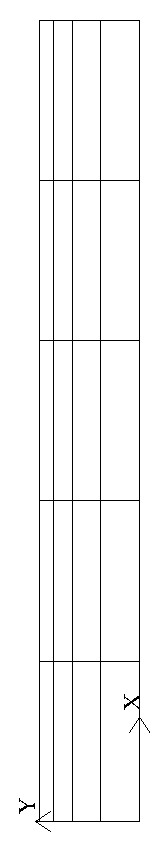
\includegraphics[width=0.8\textwidth]{Figs/mesh_axi2}
  \caption{Axisymmteric pipe mesh, graded}
  \label{fig:mesh_axi2}
\end{figure}

Suppose you wish to have the mesh be graded,
that you have increased resolution near the wall.
In this case you change {\em ratio} in the \(y\)-specification
of the element distribution.  For example, changing the 3 lines
in the above genbox input file from

\begin{verbatim}
-5 -3                         Nelx  Nely
0.0   4.0   1.0               x0  x1   ratio
0.0   0.5   1.0               y0  y1   ratio
\end{verbatim}

\noindent
to

\begin{verbatim}
-5 -4                         Nelx  Nely
0.0   4.0   1.0               x0  x1   ratio
0.0   0.5   0.7               y0  y1   ratio
\end{verbatim}

\noindent
yields the mesh shown in Fig. \ref{fig:mesh_axi2}.


\subsubsection{User-Specified Distribution}
\begin{figure}
  \centering
  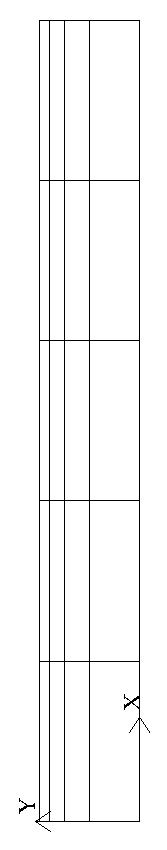
\includegraphics[width=0.6\textwidth]{Figs/mesh_axi3}
  \caption{Axisymmteric pipe mesh, user specified}
  \label{fig:mesh_axi3}
\end{figure}

You can also specify your own, precise, distribution of element
locations.   For example, another graded mesh similar to the
one of the preceding example could be built by changing the
genbox input file to contain:


\begin{verbatim}
-5  4                                               Nelx  Nely
0.0   4.0   1.0                                     x0  x1   ratio
0.000    0.250    0.375    0.450    0.500           y0  y1 ... y4
\end{verbatim}

\noindent
Here, the positive number of elements for the \(y\) direction indicates
that genbox is expecting {\tt Nely+1} values of \(y\) positions on the
\(y\)-element distribution line.   This is the genbox default, which
explains why it corresponds to {\tt Nely} \(>\) 0.  The corresponding mesh
is shown in Fig. \ref{fig:mesh_axi3}.

\subsubsection{Annulus Geometry}
\begin{verbatim}base.rea
2                         spatial dimension
2                         number of fields
Y1
-4  -8                     nelx,nely
0 0                        x0 y0 center
ccobc                      nelx+1 letter defining each edge shape
1 5 1.5                    x0 x1 ratio
0 1 1                      y0 y1 ratio
SYM,SYM,   ,               V bc's ~! NB:  3 characters each~! 
f  ,f  ,   ,               T bc's ~!      You must have 2 spaces!!
\end{verbatim}

\subsubsection{MHD}
\begin{verbatim}base.rea
3                          spatial dimensions: <0 for .re2
2.1                        number of fields       ~: v,T + B
Box 1
-4  -4  -8                 (nelx,nely,nelz for Box)
0.0 1.0 1.0                (x0, x1 ratio or xe_i)
0.0 1.0 1.0                (y0, y1 ratio or ye_j)
0.0 1.0 1.0                (z0, z1 ratio or ze_k)
P  ,P  ,P  ,P  ,P  ,P      (cbx0,  cbx1,  cby0,  cby1,  cbz0,  cbz1)  Velocity (3 characters)
P  ,P  ,P  ,P  ,P  ,P      (cbx0,  cbx1,  cby0,  cby1,  cbz0,  cbz1)  Temperature
P  ,P  ,P  ,P  ,P  ,P      (cbx0,  cbx1,  cby0,  cby1,  cbz0,  cbz1)  Magnetic Field
\end{verbatim}

\subsubsection{Cicular, 1/4 , no velocity, Passive scalars}
\begin{verbatim}base.rea
2                          spatial dimensions: <0 for .re2
-3                         number of fields       ~: (NO VELOCITY) heat + 2 passive scalars
ctest                      Signals circular geometry
0 0                        x0,y0 center
-2 -6                      nelx nely for box
1  2  1                    x0 x1 ratio
90 180 1                   y0 y1 ration~: degrees!!!!
SYM,SYM,   ,   ,           Temperature Boundary
E  ,E  ,   ,   ,           PS1
P  ,P  ,   ,   ,           PS2
\end{verbatim}


\section{Mesh Modification in Nek5000}

For complex shapes, it is often convenient to modify the mesh
direction in the simulation code, Nek5000.  This can be done
through the usrdat2 routine provided in the~.usr file.
The routine usrdat2 is called by nek5000 immediately after
the geometry, as specified by the~.rea file, is established.
Thus, one can use the existing geometry to map to a new geometry
of interest.

For example, suppose you want the above pipe geometry to have
a sinusoidal wall.  Let \(\bx := (x,y)\) denote the old geometry,
and \(\bx' := (x',y')\) denote the new geometry.  For a domain
with \(y\in [0,0.5]\), the following function will map the straight
pipe geometry to a wavy wall with amplitude \(A\), wavelength \(\lambda\):
\begin{eqnarray*}
  y'(x,y) = y  + y A \sin( 2 \pi x / \lambda ).
\end{eqnarray*}
Note that, as \(y \longrightarrow 0\), the perturbation, 
\(yA \sin( 2 \pi x / \lambda )\), goes to zero.  So, near the axis,
the mesh recovers its original form.

In nek5000, you would specify this through usrdat2 as follows


\begin{verbatim}
subroutine usrdat2
include 'SIZE'
include 'TOTAL'

real lambda

ntot = nx1*ny1*nz1*nelt

lambda = 3.
A      = 0.1

do i=1,ntot
argx         = 2*pi*xm1(i,1,1,1)/lambda
ym1(i,1,1,1) = ym1(i,1,1,1) + ym1(i,1,1,1)*A*sin(argx)
enddo

param(59) = 1.  ! Force nek5 to recognize element deformation.

return
end
\end{verbatim}
\noindent
Note that, since nek5000 is modifying the mesh, postx will not
recognize the current mesh unless you tell it to, because postx
looks to the .rea file for the mesh geometry.  The only way for
nek5000 to communicate the new mesh to postx is via the .fld
file, so you must request that the geometry be dumped to the
.fld file.   This is done by modifying the OUTPUT SPECIFICATIONS,
which are found near the bottom of the .rea file.  Specifically,
change

\begin{verbatim}
***** OUTPUT FIELD SPECIFICATION *****
6 SPECIFICATIONS FOLLOW
F      COORDINATES
T      VELOCITY
T      PRESSURE
T      TEMPERATURE
F      TEMPERATURE GRADIENT
0      PASSIVE SCALARS
\end{verbatim} 

\noindent
to

\begin{verbatim}
***** OUTPUT FIELD SPECIFICATION *****
6 SPECIFICATIONS FOLLOW
T      COORDINATES                       <------  CHANGE HERE
T      VELOCITY
T      PRESSURE
T      TEMPERATURE
F      TEMPERATURE GRADIENT
0      PASSIVE SCALARS
\end{verbatim} 

\noindent
The result of above changes is shown in Fig. \ref{fig:wavypipe}.
\begin{figure}
  \centering
  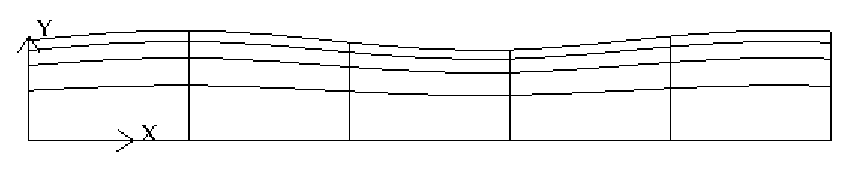
\includegraphics[width=0.8\textwidth]{Figs/wavypipe}
  \caption{Axisymmteric pipe mesh}
  \label{fig:wavypipe}
\end{figure}

\subsection{Cylindrical/Cartesian-transition Annuli}
\begin{figure}
  \centering
  \subfloat[Annuli mesh]{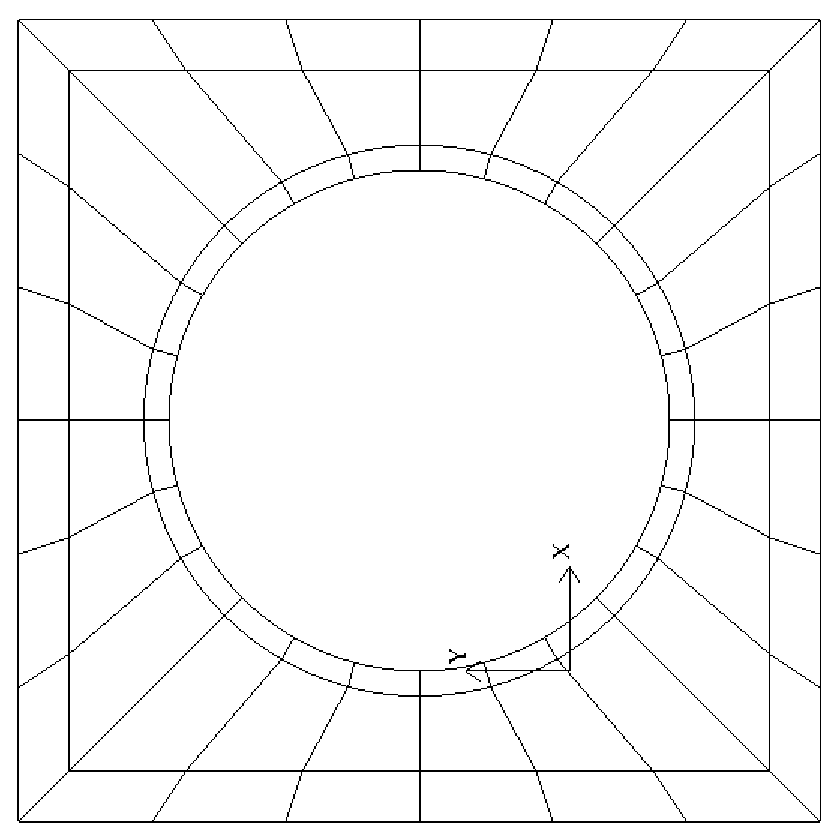
\includegraphics[width=0.3\textwidth]{Figs/cylbox_2d}\label{fig:cylbox_2d}}
  \quad\quad\quad
  \subfloat[Annuli mesh] {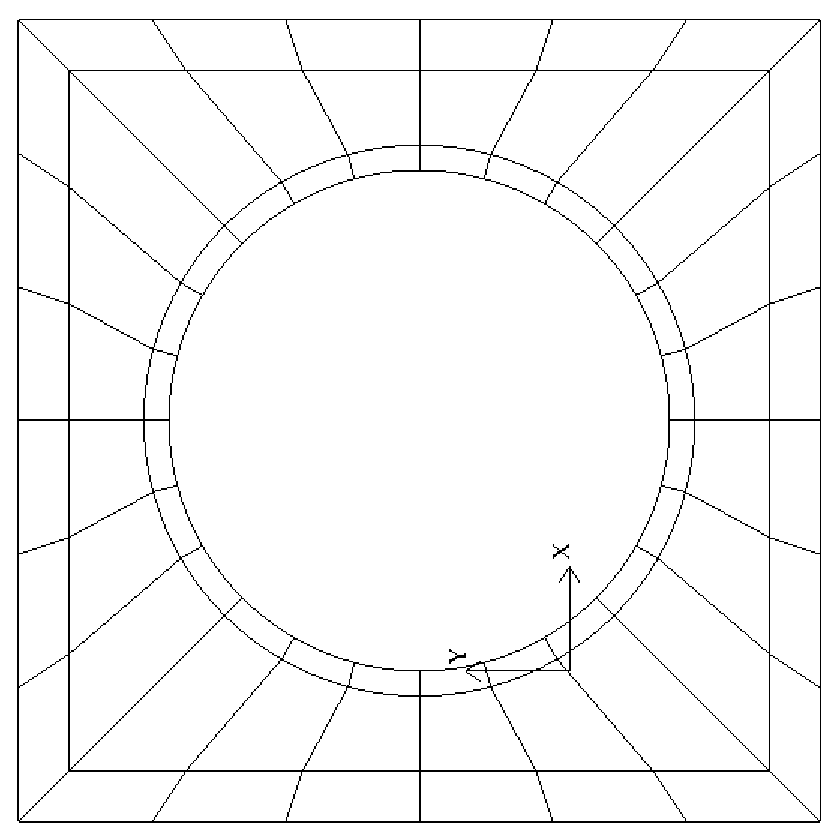
\includegraphics[width=0.3\textwidth]{Figs/cylbox_2d}\label{fig:cylbox_2da}} 
  \caption{Cylinder mesh}
\end{figure}


An updated version of genb6, known as genb7, is currently under development
and designed to simply/automate the construction of cylindrical annuli, 
including {\em basic} transition-to-Cartesian elements.   More sophisticated
transition treatments may be generated using the GLOBAL REFINE options in
prenek or through an upgrade of genb7, as demand warrants.
Example 2D and 3D input files are provided in the nek5000/doc files
{\em box7.2d} and {\em box7.3d}.
Figure \ref{fig:cylbox_2d} shows a 2D example generated using 
the {\em box7.2d} input file, which reads:
\begin{verbatim}
x2d.rea
2                      spatial dimension
1                      number of fields
#
#    comments
#
#
#========================================================
#
Y                   cYlinder
3 -24 1             nelr,nel_theta,nelz
.5 .3               x0,y0 - center of cylinder
ccbb                descriptors: c-cyl, o-oct, b-box (1 character + space)
.5 .55 .7 .8        r0 r1 ... r_nelr
0  1  1             theta0/2pi theta1/2pi  ratio 
v  ,W  ,E  ,E  ,    bc's (3 characters + comma)
\end{verbatim}

\noindent
An example of a mesh is shown in Fig. \ref{fig:cylbox_2d}.   The mesh has been quad-refined
once with oct-refine option of prenek. The 3D counterpart to this 
mesh could joined to a hemisphere/Cartesian transition built with
the spherical mesh option in prenek. 
